\section{Pianificazione}
Lo sviluppo del progetto viene organizzato e suddiviso nelle seguenti fasi:
\begin{itemize}
\item \textbf{Analisi preliminare}
\end{itemize}

\subsection{Analisi preliminare}
Questo periodo comincia nel momento in cui vengono assegnati i capitolati e termina con l'inizio di progettazione per la technology baseline.\\
\begin{center}
\textbf{periodo:} dal 5-11-2022 al 14-12-2022\\
\end{center}
In questo periodo ci concentreremo nel definire il way of working, creeremo tutta la documentazione necessaria e faremo un analisi approfondita del capitolato scelto.  Questo periodo sarà suddiviso nelle attività trattate nella seguente sezione.
\subsubsection{Attività}
\begin{itemize}
\item \textbf{Norme di progetto:} Vengono individuati gli strumenti e le linee guida da seguire durante lo sviluppo del progetto;
\item \textbf{Piano di progetto:} documento in cui vine definita la pianificazione del progetto e le sue varie fasi,  in più fornisce un preventivo per ogni fase pianificata ed il totale costo ed ore necessario per la realizzazione del progetto;
\item \textbf{Analisi dei requisti:} viene eseguito uno studio approfondito dei requisti del capitolato scelto,  di conseguenza si costruisce un diagramma dei casi d'uso e un diagramma delle attività;
\item \textbf{Glossario: } documento contenente la descrizione di termini di dominio del progetto, il glossario sarà continuamente aggiornato in base alla necessità;
\end{itemize}

\subsection{Periodi}
La fase di analisi sarà suddivisa nei seguenti periodi:
\begin{itemize}
\item \textbf{Periodo 1:} \textit{dal 5-11-2022 al 16-11-2022},  pianificazione del periodo di analisi,  suddivisone dei ruoli fra i componenti del gruppo,  prima stesura delle norme di progetto, viene effettuata un'analisi dei rischi.  Inoltre ci sarà la continua stesura di verbali dopo ogni incontro con il gruppo e con il proponente.
\item \textbf{Periodo 2:} \textit{dal 16-11-2022 al 7-12-2022},  Analisi dei requisti del capitolato scelto,  prima stesura del glossario, stesura del piano di progetto con rispettivo preventivo della fase di analisi.  I componenti del gruppo si impegnano a studiare le tecnologie necessarie per il compimento del progetto. Si continua a lavorare nei documenti redatti nei periodi precedenti e continuano ad essere prodotti verbali riguardanti le riunioni.
\item \textbf{Periodo 3: } \textit{dal 7-12-2022 al 14-12-2022} Stesura del documento analisi dei requisti. Vengono completati eventuali documenti in ritardo e avviene la verifica dei documenti che la necessitano.
\end{itemize}

\subsection{Diagramma di Gantt fase Analisi preliminare}
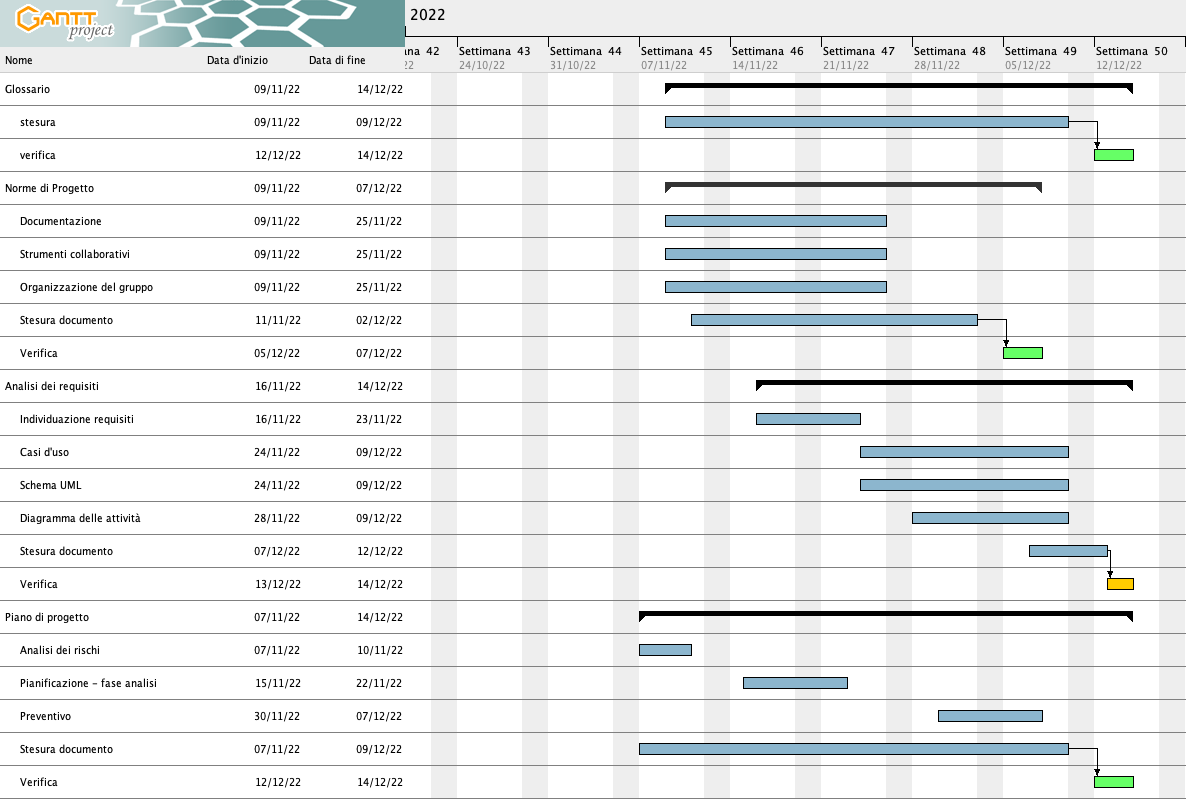
\includegraphics[scale=0.38]{image/analisi_preliminare_gantt.png}
\captionof{figure}{Diagramma di Gantt fase di analisi preliminare}
